\chapter{Desarrollo}

En esta sección se desarrollan los aspectos técnicos y conceptuales que sustentan la plataforma propuesta. En primer lugar se tratarán las bases teóricas de la criptografía simétrica y asimétrica, necesarias para comprender las decisiones de diseño posteriores. A continuación, se explicará la terminología clave y las herramientas empleadas en los flujos de actualización de los dispositivos. Finalmente, se definirá la plataforma de desarrollo propuesta y su modelo de datos.

\section{Bases teóricas de la criptografía}

En el mundo de la seguridad digital, la criptografía desempeña un papel fundamental en el cifrado y descifrado de información. Su objetivo principal es asegurar la confidencialidad e integridad de los datos, protegiéndolos contra accesos no autorizados durante la transmisión o almacenamiento. Esta sección explora los fundamentos de la criptografía, con un énfasis particular en dos formas principales: la criptografía simétrica y asimétrica.

En la criptografía, existen varios términos clave que son fundamentales para entender cómo funciona este campo. A continuación, se definen algunos de los conceptos más básicos:

\begin{itemize}
    \item \textbf{Mensaje}: Es la información original que se desea proteger.
    \item \textbf{Criptograma}: Es el resultado del proceso de cifrado, que oculta el mensaje original utilizando algún algoritmo criptográfico.
    \item \textbf{Criptoanálisis}: Es el estudio de los sistemas criptográficos con el fin de encontrar debilidades que permitan recuperar el mensaje original sin conocer la clave de cifrado.
\end{itemize}

Por otro lado, existen principios clave que son esenciales para proteger la información y los sistemas informáticos de accesos no autorizados, alteraciones y destrucción. Estos principios son la base de cualquier estrategia de seguridad y son fundamentales para garantizar la protección de los datos. A continuación, se presentan brevemente estos principios:

\begin{itemize}
    \item \textbf{Confidencialidad:} Este principio asegura que la información es accesible solo para aquellas personas autorizadas a tener acceso. Protege los datos de accesos no autorizados y garantiza la privacidad de la información.
    
    \item \textbf{Integridad:} La integridad se refiere a la exactitud y completitud de la información y los métodos de procesamiento. Este principio asegura que la información no ha sido alterada de manera no autorizada y que se mantiene tal como fue creada, enviada y recibida.
    
    \item \textbf{No repudio:} Garantiza que una vez realizada una transacción, no se pueda negar su autoría, proporcionando evidencia de la participación de las partes involucradas.
    
    \item \textbf{Autenticidad:} La autenticidad garantiza que las transacciones, las comunicaciones y los datos son genuinos y que las identidades de las partes involucradas son verificadas. Este principio evita la suplantación de identidad y asegura que los datos provienen de una fuente legítima.
\end{itemize}

\subsection{Criptografía simétrica}

La criptografía simétrica, también conocida como criptografía de clave secreta, es un método de cifrado donde se utiliza la misma clave tanto para cifrar como para descifrar la información. Esta clave debe ser compartida entre el emisor y el receptor de manera segura antes de iniciar la comunicación.

\begin{figure}[H]
    \centering
    \includegraphics[width=0.8\textwidth]{imagenes/desarrollo/sim.png}
    \caption{Uso de cifrado simétrico}
    \label{fig:cifrado_simetrico}
\end{figure}

Un ejemplo clásico de cifrado simétrico es el cifrado César, que consiste en desplazar cada letra del mensaje $n$ posiciones en el alfabeto:

\[
 E(x) = (x + n)\  \text{mod}\ {26}
\]

Asumiendo que $n$ es 1 y $x$ la posición de la letra en el abecedario, la palabra ``Hola'' pasaría a ser ``Ipmb''. En este caso, la clave sería el número de posiciones a desplazar.

La criptografía simétrica presenta ciertas limitaciones importantes:

\begin{itemize}
    \item \textbf{Distribución de claves:} La clave debe ser transmitida de manera segura entre ambas partes. Si la clave es interceptada por un tercero, toda la comunicación cifrada con esa clave se vuelve insegura.
    \item \textbf{Escalabilidad:} A medida que el número de participantes aumenta, el manejo de claves se vuelve más complejo, ya que cada par de usuarios necesita una clave única y segura.
\end{itemize}

Desde la perspectiva de la computación cuántica, el cifrado simétrico goza de una posición relativamente privilegiada. Según el NIST, algoritmos simétricos como AES-256 siguen siendo seguros a largo plazo incluso ante amenazas de computación cuántica \cite{NIST:SP800232:2023}. Esto se debe a que el algoritmo de Grover, que es el ataque cuántico más efectivo contra criptografía simétrica, reduce la seguridad efectiva a la mitad del tamaño de clave. Por ejemplo, una clave de 256 bits proporciona una seguridad equivalente a 128 bits ante un ataque cuántico, lo que sigue siendo considerado seguro por el NIST para aplicaciones sensibles.

Sin embargo, en el contexto de dispositivos IoT con recursos limitados, algoritmos como ASCON ofrecen ventajas adicionales. ASCON proporciona una variante de 80 bits de seguridad cuántica (ASCON-80pq) específicamente diseñada para resistir ataques cuánticos mientras mantiene un consumo eficiente de recursos \cite{NIST:SP800232:2023}. Esta característica lo hace particularmente atractivo para entornos donde tanto la eficiencia computacional como la resistencia cuántica son requisitos críticos.

\subsubsection{Autenticación usando cifrado simétrico: AEAD}

Para superar algunas de las limitaciones del cifrado simétrico básico y proporcionar mayor seguridad, se utilizan modos de cifrado avanzados como AEAD (Authenticated Encryption with Associated Data). AEAD combina el cifrado con la autenticación en una sola operación, garantizando tanto la confidencialidad como la integridad de los datos.

AEAD opera con tres componentes principales:
\begin{itemize}
    \item \textbf{Clave secreta:} Compartida entre emisor y receptor.
    \item \textbf{Datos a cifrar (plaintext):} El mensaje original.
    \item \textbf{Datos asociados (associated data):} Información adicional que debe autenticarse pero no cifrarse, como encabezados de protocolo.
\end{itemize}

El proceso de AEAD produce dos salidas:
\begin{itemize}
    \item \textbf{Criptograma:} Los datos cifrados.
    \item \textbf{Tag de autenticación:} Un código que verifica la integridad de los datos y los datos asociados.
\end{itemize}

Durante el descifrado, el receptor verifica el tag de autenticación. Si coincide, los datos son válidos y no han sido alterados; de lo contrario, se rechaza el mensaje. Esto previene ataques como la manipulación de datos o la repetición de mensajes.

Un ejemplo de algoritmo AEAD ampliamente utilizado es AES-GCM (Advanced Encryption Standard - Galois/Counter Mode), que combina AES para el cifrado con el modo GCM para la autenticación. Este enfoque es fundamental en protocolos seguros como TLS para proteger las comunicaciones en internet.

\subsection{Criptografía asimétrica \label{sub:crpasim}}

La criptografía asimétrica introduce un enfoque diferente mediante el uso de un par de claves: una pública y una privada. La clave pública, como su nombre indica, se puede compartir abiertamente, mientras que la clave privada se mantiene en secreto por el usuario.

La característica fundamental es que lo que es cifrado utilizando la clave pública solo puede ser descifrado por su correspondiente clave privada, y viceversa. Esta relación matemática permite establecer comunicaciones seguras sin necesidad de compartir una clave secreta previamente.

\begin{itemize}
    \item \textbf{Cifrado}: \hspace{1pt} $C = E_{k_{\text{publica}}}(M)$
    \item \textbf{Descifrado}: \hspace{1pt} $M = D_{k_{\text{privada}}}(C)$
\end{itemize}

La criptografía de clave pública y privada se puede entender mediante el símil de una caja con dos cerraduras, cada una correspondiente a una llave. Inicialmente, cualquiera de las dos llaves puede cerrar la caja, pero para abrirla se debe utilizar la llave opuesta. Imaginemos el siguiente escenario con Alice y Bob. Para este ejemplo, Bob tiene dos tipos de llaves: una pública y otra privada. La clave pública la hará disponible para todos, haciendo copias de ella y dándoselas a cualquiera que la pida. La clave privada, en cambio, será mantenida en secreto y solo Bob dispondrá de ella (ver~\autoref{fig:llaves_creadas}).

\begin{figure}[H]
    \centering
    \includegraphics[width=0.7\textwidth]{imagenes/desarrollo/bob_crea_llaves (1) (2) (1).jpg}
    \caption{Creación de las llaves por parte de Bob}
    \label{fig:llaves_creadas}
\end{figure}

\subsubsection{Cifrado con clave pública (Confidencialidad)}

\begin{enumerate}
    \item \textbf{Cerrando la caja (Encriptación con la clave pública):} Alice quiere enviar un mensaje confidencial a Bob. Para hacerlo, primero coloca el mensaje en la caja, y posteriormente utiliza la llave pública de Bob para cerrarla. Al cerrar la caja con la llave pública de Bob, Alice garantiza que solo Bob podrá abrirla, dado que solo él posee la llave privada correspondiente (ver~\autoref{fig:caja_cerr}).
    
    \begin{figure}[H]
        \centering
        \includegraphics[width=1\textwidth]{imagenes/desarrollo/alice_cierra (1).jpg}
        \caption{Alice introduce el mensaje en la caja y la cierra con la clave pública de Bob.}
        \label{fig:caja_cerr}
    \end{figure}
    
    \item \textbf{Abriendo la caja (Descifrado con la clave privada):} Cuando Bob recibe la caja cerrada, utiliza su llave privada para abrirla. Esta llave privada es única y está en su exclusiva posesión. Nadie más puede abrir la caja porque no disponen de la llave privada de Bob (ver~\autoref{fig:caja_abr}).
    
    \begin{figure}[H]
        \centering
        \includegraphics[width=0.8\textwidth]{imagenes/desarrollo/primera_parte_foto2.drawio (1).jpg}
        \caption{Bob abre la caja y obtiene el mensaje.}
        \label{fig:caja_abr}
    \end{figure}
\end{enumerate}

\subsubsection{Cifrado con clave privada (Autenticidad)}

En el ejemplo anterior se ha demostrado cómo la criptografía asimétrica puede garantizar la confidencialidad. Además, puede garantizar la autenticidad. Para ello, veamos el siguiente ejemplo donde Bob quiere enviarle un mensaje a Alice y demostrar que es Bob realmente el que lo ha escrito.

\begin{enumerate}
    \item \textbf{Cerrando la caja (Encriptación con la llave privada):} Bob coloca el mensaje en la caja y la cierra utilizando su llave privada (ver~\autoref{fig:bob_usa_priv_2}). Esto asegura que cualquier persona con acceso a su llave pública puede abrir la caja y leer el mensaje, pero garantiza que solo Bob pudo haberla cerrado, ya que solo él posee la llave privada.

    \begin{figure}[H]
        \centering
        \includegraphics[width=1\textwidth]{imagenes/desarrollo/Bob usa su clave privada.drawio (1).jpg}
        \caption{Bob inserta el mensaje y usa su llave privada.}
        \label{fig:bob_usa_priv_2}
    \end{figure}

    \item \textbf{Abriendo la caja (Descifrado con la clave pública):} Alice recibe la caja y utiliza la clave pública de Bob para abrirla (ver~\autoref{fig:alice_usa_clvpb2}). Al hacerlo, Alice puede estar segura de que el mensaje fue realmente enviado por Bob, ya que solo la llave pública de Bob puede abrir la caja que fue cerrada con su llave privada. Esto proporciona autenticidad y no repudio, ya que Bob no puede negar haber enviado el mensaje.
    
    \begin{figure}[H]
        \centering
        \includegraphics[width=0.8\textwidth]{imagenes/desarrollo/segunda parte_2.drawio (1).jpg}
        \caption{Alice utiliza la clave pública de Bob para abrir la caja y verificar la autenticidad del mensaje.}
        \label{fig:alice_usa_clvpb2}
    \end{figure}
\end{enumerate}

Mediante estos dos mecanismos, la criptografía asimétrica ofrece no solo confidencialidad, sino también no repudio y autenticidad.

\subsection{Principios de seguridad asegurados con cifrado asimétrico}

Con el cifrado asimétrico únicamente se logran los siguientes principios:

\begin{itemize}
    \item \textbf{Confidencialidad:} Se cumple, ya que el cifrado asimétrico permite proteger los datos para que solo sean accesibles por las personas autorizadas con la clave privada correspondiente.
    
    \item \textbf{Integridad:} No se puede asegurar completamente, ya que no hay un mecanismo inherente en el cifrado asimétrico que garantice que los datos no han sido alterados.
    
    \item \textbf{No repudio:} No se puede garantizar completamente, ya que el cifrado asimétrico por sí solo no proporciona una manera de evitar que una de las partes niegue haber realizado una acción.
    
    \item \textbf{Autenticidad:} No se puede asegurar completamente, ya que el cifrado asimétrico por sí solo no proporciona un método para verificar la identidad de manera confiable en una comunicación no física.
\end{itemize}

Es decir, solo podemos verificar la confidencialidad de los datos. En los siguientes apartados se verán los métodos existentes para cumplir el resto de principios.

\subsection{Firma digital}

Una firma digital es un mecanismo de seguridad electrónica que imita la funcionalidad de una firma manuscrita en el entorno digital. Utiliza la criptografía asimétrica.

Al firmar digitalmente un documento o mensaje, se utiliza la clave privada para generar un código único (la firma) basado en el contenido del mensaje mediante una función hash\footnote{Una función hash convierte datos de cualquier tamaño en una cadena de texto de tamaño fijo, conocida como hash. Cada conjunto único de datos produce un hash único, y cualquier cambio en los datos cambia el hash.}. Este código se adjunta después al mensaje o documento. Cuando el receptor obtiene el mensaje firmado, puede usar la clave pública del remitente para verificar si la firma es válida.

Para crear la firma se siguen los siguientes pasos:
\begin{itemize}
    \item \textbf{Creación del hash}: Primero, el remitente crea un resumen del mensaje original utilizando una función hash criptográfica. 
    \item \textbf{Firmado del hash}: A continuación, el remitente cifra el hash del mensaje con su clave privada. La firma digital no es el cifrado completo del mensaje, sino el cifrado del hash del mensaje.
    \item \textbf{Adjuntar al mensaje}: El hash cifrado (la firma) se adjunta al mensaje original. Este mensaje firmado se puede enviar al receptor.
\end{itemize}

Y para verificar la firma:
\begin{itemize}
    \item \textbf{Separar la firma y el mensaje}.
    \item \textbf{Descifrar la firma}: El receptor utiliza la clave pública del remitente para descifrar la firma, obteniendo así el hash del mensaje que el remitente calculó.
    \item \textbf{Calcular el hash del mensaje}: El receptor calcula el hash del mensaje recibido utilizando la misma función hash que usó el remitente.
    \item \textbf{Comparar los hashes}: El receptor compara el hash que acaba de calcular con el hash descifrado de la firma. Si ambos hashes coinciden, la firma es válida; esto significa que el mensaje no ha sido alterado y que el remitente es quien dice ser.
\end{itemize}

De esta manera se puede garantizar la autenticidad, la integridad y el no repudio:

\begin{itemize}
    \item \textbf{Integridad}: Si la verificación es exitosa, se puede estar seguro de que el mensaje no ha sido alterado desde que fue firmado.
 
    \item \textbf{Autenticidad}: Al verificar con éxito la firma digital, se confirma que el mensaje fue realmente enviado por quien posee la clave privada correspondiente.

    \item \textbf{No Repudio}: Una vez enviado un mensaje firmado digitalmente, el remitente no puede negar haberlo enviado, ya que la firma digital creada con su clave privada es única y verificable por cualquier persona que tenga su clave pública.
\end{itemize}

Al combinar esto con el cifrado asimétrico convencional, también se garantiza la confidencialidad. Sin embargo, la autenticidad completa solo se puede lograr con la introducción de autoridades certificadoras (CA), que se discutirá a continuación.

\subsection{Autoridades Certificadoras y certificados digitales}

En las comunicaciones digitales, es crucial garantizar que las partes involucradas sean quienes dicen ser. Aquí es donde entra en juego la Autoridad Certificadora (CA). Una CA es una entidad de confianza que emite certificados digitales, los cuales verifican la identidad de los individuos, servidores u otras entidades. Sin una CA, sería muy difícil establecer una relación de confianza en entornos donde las partes no se conocen previamente.

\subsubsection{Autoridad Certificadora}

Una Autoridad Certificadora (CA) es una organización responsable de emitir y gestionar certificados digitales. La CA actúa como un tercero de confianza en el ecosistema de la infraestructura de clave pública (PKI). Su papel principal incluye:

\begin{itemize}
    \item Verificar la identidad de las entidades que solicitan un certificado digital.
    \item Emitir certificados digitales que enlazan una clave pública con la identidad del solicitante.
    \item Revocar certificados digitales si ya no son válidos o se comprometen.
    \item Publicar listas de certificados revocados (CRL).
\end{itemize}

\subsubsection{Certificado digital}

Un certificado digital es un documento electrónico que utiliza una firma digital para enlazar una clave pública con la identidad del propietario del certificado. Esto se consigue firmando la clave pública del propietario del certificado con la clave privada de la autoridad certificadora. Un certificado digital contiene varios campos clave:

\begin{itemize}
    \item \textbf{Nombre del propietario}: Identifica al propietario del certificado.
    \item \textbf{Clave pública del propietario}: La clave pública asociada con el propietario.
    \item \textbf{Nombre de la CA}: La entidad que emitió el certificado.
    \item \textbf{Firma digital de la CA}: La firma digital de la CA que valida el certificado.
    \item \textbf{Período de validez}: Las fechas de inicio y expiración del certificado.
    \item \textbf{Número de serie del certificado}: Un número único para identificar el certificado.
\end{itemize}

Los certificados digitales siguen el estándar X.509, que establece el formato y las reglas para su emisión y procesamiento en sistemas de infraestructura de clave pública (PKI).

\subsubsection{Proceso de Verificación de Certificados}

\begin{enumerate}
    \item \textbf{Firma del Certificado}: La CA utiliza su clave privada para firmar el certificado digital del propietario.
    \item \textbf{Verificación del Certificado}: Cualquier entidad que reciba el certificado puede usar la clave pública de la CA (generalmente disponible y conocida) para verificar la firma del certificado. Si la verificación es exitosa, se confía en la identidad del propietario del certificado.
\end{enumerate}

\subsubsection{Jerarquía de las Autoridades Certificadoras}

Las CA se organizan en una jerarquía, donde las CA de nivel superior, la CA raíz (root CA), firman los certificados de las CA subordinadas (CA intermedio), y estas, a su vez, pueden firmar certificados para usuarios finales o servidores. Esto crea una cadena de confianza que puede ser verificada siguiendo el camino desde un certificado de usuario final hasta la raíz CA.

En la \autoref{fig:ca-hierarchy}, se presenta un diagrama que ilustra esta jerarquía:

\begin{figure}[H]
\centering
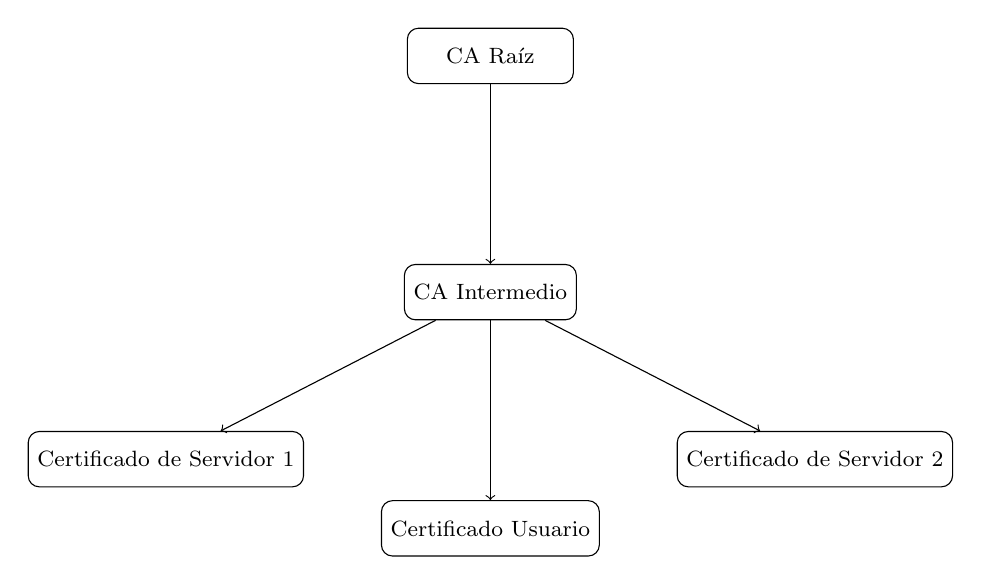
\begin{tikzpicture}[node distance=3cm, auto]

\tikzstyle{every node}=[font=\footnotesize]
\tikzstyle{ca} = [rectangle, draw, text centered, rounded corners, minimum height=2em, minimum width=6em]

% Nodos
\node[ca] (rootca) {CA Raíz};
\node[ca, below of=rootca] (intermediateca) {CA Intermedio};
\node[ca, below left of=intermediateca, xshift=-2cm] (servercert1) {Certificado de Servidor 1};
\node[ca, below right of=intermediateca, xshift=2cm] (servercert2) {Certificado de Servidor 2};
\node[ca, below of=intermediateca] (usercert) {Certificado Usuario};

% Lines
\draw[->] (rootca) -- (intermediateca);
\draw[->] (intermediateca) -- (servercert1);
\draw[->] (intermediateca) -- (servercert2);
\draw[->] (intermediateca) -- (usercert);

\end{tikzpicture}
\caption{Jerarquía de las Autoridades Certificadoras.}
\label{fig:ca-hierarchy}
\end{figure}

\section{Elección de algoritmos criptográficos}

Para este proyecto, la selección de algoritmos criptográficos se ha basado en las necesidades actuales del ecosistema IoT y en la gran diversidad de dispositivos que lo componen. El panorama IoT abarca desde microcontroladores con recursos extremadamente limitados (pocos kilobytes de RAM y MHz de procesamiento) hasta dispositivos más potentes como gateways o sistemas embebidos basados en Linux. Esta heterogeneidad hace inviable la adopción de una única solución criptográfica que se adapte óptimamente a todos los escenarios.

Actualmente, el estándar de facto para el cifrado simétrico es AES (Advanced Encryption Standard). Este algoritmo es extremadamente robusto y eficiente en plataformas que disponen de recursos suficientes, especialmente aquellas que cuentan con aceleración por hardware (instrucciones AES-NI o similares). Sin embargo, en dispositivos restringidos sin soporte hardware específico, la implementación de AES puede resultar costosa en términos de ciclos de reloj, consumo de energía y uso de memoria, además de ser susceptible a ataques de canal lateral si no se implementa con complejas contramedidas.

En el ámbito de la criptografía asimétrica, y específicamente en lo referente a la firma digital, los estándares actuales más utilizados son RSA y ECDSA. Este último, basado en curvas elípticas, destaca por su eficiencia frente a RSA, permitiendo longitudes de clave mucho menores para un mismo nivel de seguridad. Adicionalmente, en este proyecto se tiene la intención de añadir soporte para MLDSA (Module-Lattice-Based Digital Signature Standard), un algoritmo de firma post-cuántica que será detallado más adelante.

Por esta razón, se ha decidido ofrecer soporte para múltiples familias de algoritmos, permitiendo que cada despliegue seleccione la opción más adecuada según las capacidades del hardware objetivo. 

\subsection{ASCON: Estándar de criptografía ligera}

ASCON ha sido seleccionado por el NIST (National Institute of Standards and Technology) como el estándar oficial de criptografía ligera para dispositivos con recursos limitados, publicado en la especificación NIST SP 800-232 \cite{NIST:SP800232:Ascon}. Esta selección consiste en un proceso de evaluación de varios años en el que ASCON demostró un equilibrio óptimo entre seguridad, eficiencia y versatilidad.

ASCON es una familia de algoritmos que proporciona:
\begin{itemize}
    \item \textbf{Cifrado autenticado (AEAD):} Garantiza confidencialidad e integridad en una sola operación.
    \item \textbf{Funciones hash:} Para verificación de integridad y generación de resúmenes criptográficos.
    \item \textbf{Autenticación de mensajes (MAC):} Para verificar la autenticidad sin cifrado.
\end{itemize}

Ascon cuenta con 3 variantes principales:

\begin{itemize}
    \item \textbf{Ascon-128:} La variante estándar que ofrece 128 bits de seguridad simétrica. Ideal para la mayoría de las aplicaciones IoT.
    \item \textbf{Ascon-128a:} Versión alternativa de alto rendimiento, que sacrifica ligeramente el tamaño del código por una mayor velocidad de procesamiento.
    \item \textbf{Ascon-80pq:} Variante de seguridad post-cuántica (post-quantum), diseñada con una clave de 160 bits para abordar desafíos de seguridad futuros.
\end{itemize}


\subsubsection{Ventajas de rendimiento frente a AES}

Según los benchmarks realizados por los autores de ASCON en el documento \textit{Status Update on Ascon v1.2} \cite{AsconStatusUpdate2022}, el algoritmo presenta ventajas significativas en dispositivos sin aceleración hardware para AES:

\begin{itemize}
    \item \textbf{Velocidad:} ASCON es entre 2 y 5 veces más rápido que AES-GCM en implementaciones software sobre microcontroladores de 8, 16 y 32 bits sin instrucciones AES dedicadas.
    \item \textbf{Tamaño de código:} La implementación de ASCON requiere significativamente menos memoria de programa que AES, lo cual es crítico en dispositivos con flash limitada.
    \item \textbf{Uso de RAM:} El estado interno de ASCON (320 bits) es compacto, reduciendo el consumo de memoria durante las operaciones criptográficas.
    \item \textbf{Tamaño de clave:} ASCON opera con claves de 128 bits, ofreciendo un nivel de seguridad adecuado teniendo en cuenta el objetivo de este, la criptografía ligera.
\end{itemize}

\subsubsection{Validación experimental}

Para validar la elección de ASCON, se decidió realizar pruebas experimentales en dos dispositivos representativos de entornos IoT con recursos limitados y sin aceleración por hardware para criptografía: una Raspberry Pi 3 \cite{RaspberryPi:Website} y un Arduino UNO R4 \cite{ArduinoIDE:Website}.

La implementación utilizada para las pruebas es la oficial de ASCON (versión 1.3.0) disponible en GitHub \cite{ASCON:Code:2023}, la cual es la recomendada por el NIST \cite{NIST:Website}.

Las pruebas en la Raspberry Pi 3 han consistido en el cifrado y descifrado de un fichero de 100 MB. Para asegurar la fiabilidad de los datos y reducir la variabilidad, se ejecutaron 100 iteraciones de cada prueba.

En el caso del Arduino, debido a las limitaciones inherentes de un microcontrolador, las pruebas fueron más restringidas. Se procedió probando con tamaños de texto plano (\textit{plaintext}) incrementales, desde pocos bytes hasta el límite permitido por la memoria del dispositivo.

Los resultados obtenidos para la Raspberry Pi 3 se muestran en la \autoref{fig:rpi_results}.

\begin{figure}[H]
    \centering
    \includegraphics[width=1\textwidth]{imagenes/desarrollo/rpi_results.png}
    \caption{Resultados de rendimiento en Raspberry Pi 3}
    \label{fig:rpi_results}
\end{figure}

Como se puede observar, ASCON confirma su superioridad frente a las variantes de AES, siendo entre 2 y 5 veces más rápido en este entorno sin aceleración hardware. Además, su rendimiento es equiparable al de ChaCha20-Poly1305, otro algoritmo conocido por su eficiencia en software.

Por otro lado, en el entorno más restringido del Arduino, los resultados son mucho más favorables para ASCON en todos los sentidos, como se aprecia en la \autoref{fig:arduino_results}.

\begin{figure}[H]
    \centering
    \includegraphics[width=0.8\textwidth]{imagenes/desarrollo/arduino_results.png}
    \caption{Resultados de rendimiento en Arduino UNO R4}
    \label{fig:arduino_results}
\end{figure}

ASCON resulta ser el claro ganador. Además, es importante destacar la eficiencia en el uso de memoria. En la \autoref{fig:max_plaintext_arduino} se muestra cómo ASCON permite cifrar y descifrar bloques de texto plano más grandes que el resto de algoritmos antes de agotar los recursos del microcontrolador, lo cual se atribuye a su menor consumo de memoria RAM.

\begin{figure}[H]
    \centering
    \includegraphics[width=0.8\textwidth]{imagenes/desarrollo/max_plaintext_arduino.png}
    \caption{Tamaño máximo de texto plano admitido en Arduino}
    \label{fig:max_plaintext_arduino}
\end{figure}

Adicionalmente, al considerar el uso de ASCON como algoritmo AEAD, el tamaño del tag y los bytes adicionales que se añaden al texto plano son aspectos cruciales a evaluar. En la \autoref{fig:tag_tamaño} se ilustra la cantidad de bytes extra requeridos por cada algoritmo en comparación con el texto plano original. ASCON ocupa la mejor posición con solo 16 bytes adicionales, junto con AES-CTR y ChaCha20 sin autenticación.

\begin{figure}[H]
    \centering
    \includegraphics[width=0.8\textwidth]{imagenes/desarrollo/tag_tamaño.png}
    \caption{Bytes adicionales requeridos por algoritmos AEAD}
    \label{fig:tag_tamaño}
\end{figure}

\subsubsection{Consideraciones de seguridad post-cuántica}

Más allá de las ventajas de rendimiento, ASCON ofrece también protección contra amenazas futuras derivadas del desarrollo de computadores cuánticos. Según el NIST, algoritmos simétricos como AES-256 siguen siendo seguros a largo plazo incluso ante amenazas de computación cuántica \cite{NIST:SP800232:2023}. Esto se debe a que el algoritmo de Grover, que es el ataque cuántico más efectivo contra criptografía simétrica, reduce la seguridad efectiva a la mitad del tamaño de clave. Por ejemplo, una clave de 256 bits proporciona una seguridad equivalente a 128 bits ante un ataque cuántico, lo que sigue siendo considerado seguro por el NIST para aplicaciones sensibles.

Sin embargo, ASCON-80pq proporciona una protección algo más robusta. Esta variante está específicamente diseñada con una clave de 160 bits para garantizar 80 bits de seguridad efectiva incluso ante ataques cuánticos basados en el algoritmo de Grover \cite{NIST:SP800232:2023}. Si bien no es la variante más recomendada para entornos con recursos abundantes, donde AES-256 ofrecería una mayor seguridad a largo plazo, no está mal considerada, especialmente en dispositivos con recursos limitados o en entornos IoT donde la eficiencia computacional es un factor crítico. Esta característica lo hace particularmente atractivo para entornos IoT donde tanto la eficiencia computacional como la resistencia cuántica a largo plazo son requisitos críticos.

\subsubsection{Seguridad post cuantica en la firma digital: MLDSA}

El panorama es significativamente diferente en el caso de la criptografía asimétrica. El algoritmo de Shor \cite{shor1997}, propuesto en 1997, demostró teóricamente que los sistemas criptográficos asimétricos actuales, como RSA y ECDSA, son completamente vulnerables a un computador cuántico suficientemente potente. Este algoritmo puede factorizar números grandes y resolver logaritmos discretos en tiempo polinómico, haciendo que los métodos de clave pública actuales sean obsoletos ante una amenaza cuántica.

En respuesta a esta amenaza, el NIST ha recomendado la transición hacia algoritmos basados en retículos (lattice-based cryptography). Para firmas digitales, el estándar recomendado es MLDSA (Module-Lattice-Based Digital Signature Algorithm), estandarizado en el FIPS 204 \cite{NIST:FIPS204}. MLDSA ofrece seguridad matemáticamente resistente a ataques cuánticos mientras mantiene una eficiencia computacional aceptable para la mayoría de aplicaciones, incluyendo dispositivos con recursos limitados.

Si bien la transición no es urgente, dado que actualmente no existen computadores cuánticos capaces de ejecutar el algoritmo de Shor a escala práctica y todas las firmas verificadas hoy en día permanecen seguras, realizar el salto hacia algoritmos post-cuánticos es altamente recomendado para garantizar la seguridad a largo plazo.

La combinación de cifrado simétrico resistente a la computación cuántica (ASCON-80pq para confidencialidad) con firmas digitales basadas en retículos (MLDSA para autenticidad) constituye un enfoque integral para garantizar la seguridad criptográfica a largo plazo, tanto ante amenazas actuales como futuras.

\section{Actualizaciones de software en sistemas embebidos}

La capacidad de actualizar el software de manera remota y segura (OTA - Over-The-Air) nos permiten, no solo corregir errores y vulnerabilidades de seguridad, sino también desplegar nuevas funcionalidades durante la vida útil del dispositivo.

Para comprender el diseño del sistema de actualizaciones propuesto, es necesario definir primero algunos conceptos clave del ecosistema Linux embebido.

\subsection{Conceptos fundamentales}

\subsubsection{Yocto Project}

El Proyecto Yocto es un proyecto de colaboración de código abierto que ayuda a los desarrolladores a crear sistemas personalizados basados en Linux para productos embebidos, independientemente de la arquitectura del hardware. Proporciona un conjunto flexible de herramientas y un espacio en el que los desarrolladores de sistemas embebidos de todo el mundo pueden compartir tecnologías, pilas de software, configuraciones y mejores prácticas que se pueden utilizar para crear imágenes de Linux personalizadas para dispositivos embebidos.

En la terminología de Yocto, se definen conceptos clave como \textit{recipes} (recetas), que son archivos que describen cómo obtener, configurar, compilar e instalar un paquete de software, y \textit{layers} (capas), que agrupan recetas relacionadas. Este sistema permite generar imágenes de sistema completas, incluyendo el bootloader, el kernel y el rootfs, de manera reproducible y controlada.

\subsubsection{Bootloader}

El \textit{bootloader} o gestor de arranque es el primer programa que se ejecuta cuando se enciende el dispositivo. Su responsabilidad principal es inicializar el hardware esencial (CPU, memoria RAM, relojes) y cargar el sistema operativo (kernel de Linux) en la memoria para su ejecución.

En el contexto de las actualizaciones OTA, el bootloader juega un papel crítico: es el componente encargado de decidir qué partición del sistema operativo se debe arrancar. Esto permite, por ejemplo, arrancar desde una nueva versión del software tras una actualización exitosa o volver a la versión anterior si la nueva falla. U-Boot (Universal Boot Loader) es el estándar de facto en sistemas Linux embebidos debido a su flexibilidad y soporte para múltiples arquitecturas.

\subsubsection{Rootfs (Sistema de archivos raíz)}

El \textit{rootfs} o sistema de archivos raíz es la estructura de directorios que contiene todos los archivos necesarios para que el sistema operativo funcione, incluyendo bibliotecas, binarios, archivos de configuración y las aplicaciones del usuario. En sistemas embebidos robustos, es común que el rootfs se monte en modo de solo lectura (\textit{read-only}) durante la operación normal. Esto protege la integridad del sistema frente a cortes de energía repentinos o corrupción de datos, asegurando que el dispositivo siempre arranque en un estado conocido.

\subsubsection{Estrategia de actualización A/B}

La estrategia de actualización A/B, también conocida como de doble partición o \textit{dual-copy}, es el mecanismo más robusto para garantizar actualizaciones seguras y atómicas. El almacenamiento del dispositivo se divide en dos conjuntos idénticos de particiones (Slot A y Slot B) para el sistema operativo (kernel y rootfs).

El funcionamiento es el siguiente:
\begin{itemize}
    \item El dispositivo arranca y opera desde una de las particiones (por ejemplo, Slot A), que se considera la partición "activa".
    \item Cuando se recibe una actualización, esta se instala en la partición inactiva (Slot B), sin interrumpir el funcionamiento del sistema.
    \item Una vez completada la instalación, se instruye al bootloader para que intente arrancar desde el Slot B en el próximo reinicio.
    \item Si el arranque del Slot B es exitoso, se marca como la nueva partición activa. Si falla (por ejemplo, el sistema se cuelga o no pasa los tests de arranque), el bootloader revierte automáticamente al Slot A, garantizando que el dispositivo siga operativo.
\end{itemize}

Este mecanismo proporciona redundancia y asegura que el dispositivo nunca quede inutilizado por una actualización fallida o corrupta, como se ilustra en la Figura~\ref{fig:ab_install}.

\begin{figure}[h]
\centering
\includegraphics[width=0.8\textwidth]{imagenes/desarrollo/AB_install.png}
\caption{Proceso de instalación de actualización A/B.}
\label{fig:ab_install}
\end{figure}

\subsection{SWUpdate: Gestor de actualizaciones}

SWUpdate es un framework de actualización de software de código abierto diseñado específicamente para sistemas Linux embebidos. A diferencia de gestores de paquetes tradicionales como \textit{apt} o \textit{dnf}, que actualizan archivos individuales, SWUpdate está orientado a la actualización de imágenes completas del sistema o particiones, lo cual es ideal para garantizar la consistencia en dispositivos IoT. Cabe destacar que SWUpdate es una de las soluciones recomendadas por el Proyecto Yocto para realizar actualizaciones de sistema completas y seguras \cite{Yocto:SystemUpdate}.

SWUpdate actúa como un agente que se ejecuta en el dispositivo y gestiona todo el proceso de actualización. Sus principales características y cualidades incluyen:

\begin{itemize}
    \item \textbf{Soporte para actualizaciones A/B:} Se integra nativamente con el bootloader (como U-Boot) para gestionar el cambio de particiones y el mecanismo de \textit{fallback} en caso de fallo.
    \item \textbf{Actualizaciones atómicas:} Garantiza que el sistema se actualice completamente o no se actualice en absoluto, evitando estados inconsistentes.
    \item \textbf{Streaming:} Permite instalar la actualización mientras se descarga, sin necesidad de almacenar el archivo completo en el almacenamiento local. Esto es crucial en dispositivos con memoria flash limitada.
    \item \textbf{Seguridad:} Soporta la verificación de imágenes firmadas digitalmente (utilizando RSA, CMS o claves simétricas) y el descifrado de imágenes, asegurando que solo software auténtico y autorizado pueda ser instalado.
    \item \textbf{Flexibilidad:} Es altamente configurable y soporta múltiples fuentes de actualización (USB, red, OTA) y formatos de imagen (raw, comprimidos con zstd/gzip, etc.).
\end{itemize}

En este proyecto, SWUpdate se utiliza como el componente central en el lado del dispositivo para orquestar la descarga, verificación e instalación de las nuevas versiones de firmware.

\subsubsection{Arquitectura modular}

Una de las características más destacadas de SWUpdate es su arquitectura altamente modular. El sistema dispone de gran cantidad de módulos o "handlers" que permiten gestionar diferentes tipos de artefactos (imágenes de disco, archivos, scripts, bootloaders) y comunicarse con diversos backends de gestión (SurBit, Hawkbit, servidores web genéricos, etc.).

En este proyecto en específico, se ha hecho uso del módulo \textbf{WFX} \cite{WFX}. Este módulo actúa como unión con el gestor de actualizaciones central c, encargándose de la comunicación con la plataforma de gestión en la nube donde WFX está ejecutado. A través del módulo WFX, el dispositivo puede consultar la disponibilidad de nuevas versiones, descargar los paquetes de actualización y reportar el estado final del proceso. El módulo WFX tiene soporte para dos tipos de actualizaciones: directo y por fases, donde el segundo requiere actividad del desarrollador. De todos modos, esto se detallará más en profundidad en la siguiente sección en conjunto con la herramienta WFX.

\subsubsection{Formato de paquete .swu y descriptor}

El paquete de actualización que maneja SWUpdate es un archivo con extensión \texttt{.swu}. Técnicamente, un archivo \texttt{.swu} es un contenedor en formato CPIO (\textit{Copy In, Copy Out}) que agrupa todos los elementos necesarios para la actualización. Dentro de este contenedor se encuentran:

\begin{itemize}
    \item \textbf{Imágenes de software:} Los binarios, sistemas de archivos o archivos individuales que se van a instalar (por ejemplo, imágenes \textit{raw} o archivos de firmware).
    \item \textbf{Scripts:} Scripts de pre-instalación o post-instalación si son necesarios.
    \item \textbf{Descriptor (sw-description):} El archivo más importante, que describe el contenido del paquete y las reglas de instalación.
\end{itemize}

El archivo \texttt{sw-description} utiliza una sintaxis basada en \textit{libconfig} y define metadatos como la versión, compatibilidad de hardware y la lista de archivos a instalar. A continuación se muestra un ejemplo de un descriptor básico:

\begin{verbatim}
software =
{
        version = "1.2";
        reboot = false;
        description = "Update vnull - OTA patch";
        hardware-compatibility: [ "1.0", "1.2", "1.3" ];

        ecs = {
                files: (
                        {
                                filename = "fichero";
                                path = "/ruta/fichero";
                                type = "rawfile";
                        }
                );
        }
}
\end{verbatim}

En este ejemplo, se define una actualización versión \enquote{1.2} compatible con varias revisiones de hardware. La sección \texttt{ecs} (que podría ser cualquier nombre de agrupación) contiene una lista de archivos, en este caso un único archivo de tipo \texttt{rawfile} que se copiará a la ruta especificada.

\subsubsection{Flujo de actualización (Pulling)}

El proceso de actualización en este proyecto sigue un modelo de "pulling" (sondeo), donde la iniciativa parte del dispositivo. El funcionamiento típico con el gestor de actualizaciones es el siguiente:

\begin{enumerate}
    \item \textbf{Comprobación (Polling):} El servicio SWUpdate en el dispositivo consulta periódicamente al servidor central (a través del módulo WFX) si existe una nueva actualización disponible para su versión de hardware y software actual.
    \item \textbf{Descarga:} Si el servidor responde afirmativamente con una actualización pendiente, el dispositivo comienza la descarga del archivo \texttt{.swu}.
    \item \textbf{Instalación:} SWUpdate procesa el archivo \texttt{.swu}, lee el descriptor \texttt{sw-description} y procede a instalar los artefactos según las reglas definidas.
    \item \textbf{Confirmación:} Una vez finalizada la instalación, el dispositivo reporta el éxito o fracaso de la operación al servidor.
\end{enumerate}

\subsection{WFX: Workflow Executioner}

WFX (\textit{Workflow Executioner}) es una herramienta desarrollada por Siemens y escrita en el lenguaje de programación Go, diseñada para gestionar la ejecución de flujos de trabajo (\textit{workflows}) en entornos distribuidos. En el contexto de este proyecto, WFX actúa como el gestor del sistema de actualizaciones OTA, orquestando el ciclo de vida de las actualizaciones desde que se definen hasta que se instalan en los dispositivos.

El funcionamiento de WFX se basa en máquinas de estados cliente-servidor. Un flujo de trabajo define una serie de estados por los que debe pasar una tarea (en este caso, una actualización) y las transiciones permitidas entre ellos. Estas transiciones pueden ser desencadenadas por el dispositivo (el cliente, a través de SWUpdate) o por el operador del sistema (el desarrollador o administrador).

Para facilitar esta interacción, WFX expone dos APIs diferenciadas:
\begin{itemize}
    \item \textbf{API Norte (North API):} Destinada al desarrollador o a los sistemas de gestión. Permite crear trabajos, monitorizar su estado y ejecutar transiciones administrativas (como aprobar una actualización).
    \item \textbf{API Sur (South API):} Destinada a los dispositivos. Es utilizada por el agente SWUpdate (a través del módulo WFX) para consultar tareas pendientes, reportar progreso y actualizar el estado de la instalación.
\end{itemize}

\subsubsection{Tipos de Workflows}

WFX integra flujos de trabajo específicos para la actualización de artefactos en dispositivos, conocidos como DAU (\textit{Device Artifact Update}). El sistema soporta dos modalidades principales: \textit{Direct} (Directo) y \textit{Phased} (Por fases).

\paragraph{Workflow Directo}

El \textbf{Workflow Directo} es un proceso automatizado diseñado para despliegues rápidos donde no se requiere intervención manual. Una vez creado el trabajo, el dispositivo procede a la descarga e instalación sin pausas intermedias, como se muestra en la Figura \ref{fig:workflow_direct}.

\begin{figure}[h]
    \centering
    \includegraphics[width=0.4\textwidth]{imagenes/desarrollo/direct.png}
    \caption{Diagrama de estados del Workflow Directo.}
    \label{fig:workflow_direct}
\end{figure}

\paragraph{Workflow Por Fases}

El \textbf{Workflow Por Fases} introduce puntos de control manual para una gestión más controlada del despliegue. Es fundamental notar los estados marcados con los símbolos \texttt{<>} en el diagrama de la Figura \ref{fig:workflow_phased}. Estos estados indican que la transición no es automática, sino que requiere una acción explícita por parte del desarrollador a través de la API Norte. Específicamente, estas intervenciones son necesarias para dar inicio a la actualización y para activarla una vez instalada, permitiendo un control granular sobre el despliegue (por ejemplo, para coordinar reinicios en ventanas de mantenimiento).

\begin{figure}[H]
    \centering
    \includegraphics[width=0.4\textwidth]{imagenes/desarrollo/phased.png}
    \caption{Diagrama de estados del Workflow Por Fases.}
    \label{fig:workflow_phased}
\end{figure}

\subsubsection{La Entidad Job}

En la arquitectura de WFX, cuando se asigna una actualización a un dispositivo, se crea una entidad denominada \textbf{Job} (Trabajo). El agente SWUpdate en el dispositivo sondea constantemente la API Sur de WFX buscando si existe algún \textit{Job} activo asignado a su \textit{DeviceID}.

Un \textit{Job} encapsula toda la información necesaria para realizar la actualización, tal y como se ilustra en la Figura \ref{fig:job_definition}. Sus componentes principales son:

\begin{figure}[h]
    \centering
    \includegraphics[width=0.6\textwidth]{imagenes/desarrollo/job_definition.png}
    \caption{Estructura de la entidad Job en WFX.}
    \label{fig:job_definition}
\end{figure}

\begin{itemize}
    \item \textbf{ID:} Identificador único del trabajo.
    \item \textbf{DeviceID:} Identificador del dispositivo al que está asignado el trabajo.
    \item \textbf{Workflow:} Nombre del flujo de trabajo que rige este trabajo (ej. \texttt{wfx.workflow.dau.direct}).
    \item \textbf{Tags:} Etiquetas para categorización y búsquedas.
    \item \textbf{State:} Estado actual del trabajo dentro del flujo (ej. \texttt{CREATED}, \texttt{DOWNLOADING}, \texttt{INSTALLED}).
    \item \textbf{Progress:} Indicador numérico del progreso de la tarea.
    \item \textbf{Message:} Mensajes de log o errores reportados por el dispositivo.
    \item \textbf{Hash:} Valor hash para identificar y verificar la integridad del trabajo.
    \item \textbf{Fechas:} \textit{Start time} (inicio) y \textit{Modification time} (última actualización).
    \item \textbf{History:} Un registro histórico en formato JSON que almacena la evolución del trabajo, incluyendo cambios de estado, tiempos de modificación y mensajes.
\end{itemize}

Un componente crítico del \textit{Job} es el campo \textbf{Definition} (metadatos). Este campo se almacena como un objeto JSON y contiene los detalles técnicos de la actualización que el dispositivo necesita procesar. En este proyecto, el campo \textit{Definition} se ha utilizado para inyectar identificadores y configuraciones específicas:

\begin{itemize}
    \item \textbf{Artifacts:} Lista de objetos a instalar. Cada artefacto incluye un \textbf{Name} y una \textbf{Uri} (ruta de descarga).
    \item \textbf{Version:} Versión del paquete de software.
    \item \textbf{Type:} Tipo de actualización.
    \item \textbf{DMSID y LaunchID:} Etiquetas utilizadas como identificadores únicos para búsquedas y trazabilidad dentro del sistema de gestión.
\end{itemize}